\chapter{Discussion}
We decided to start this project because parser construction is an interesting
subject, and because the outcome, if successfull, would have real world
applicability. The rationale for writing a new parser instead of using an
existing one is simple - as shown in section \ref{sect:theory:stateoftheart},
current full-text implementations are tightly coupled with their
host environment and unsuitable for integration with new backends, limited by
restrictive licenses, or simply available only in platform-dependent binaries
(as opposed to Java). 

In this chapter, we will discuss the outcome of this project and reflect over
our decisions. We will present and evaluate alternative decisions, and what
might have come of them. We will also discuss problems, how they were
solved, and attempt to reflect over how these problems could have been solved
differently.

\section{Design Decisions}
\label{sect:discussion:designDecisions}

Of the alternatives in section \ref{sect:ambiguousgrammar:ambigTerm}, we ended up, as previously mentioned, on the parser controlled state driven lexer alternative. This strategy depends upon the lexer not generating any tokens before they are needed by the parser, dealt with by our implementation of \verb!UnbufferedCommonTokenStream!, and that most terminal alternatives are augmented with semantic predicates controlling which alternatives are available in which state.

\subsection{Parser Controlled Lexer}
Making the lexer emit one and one token instead of processing the input as a
whole, most probably leads to a slightly prolonged execution time as the
runtime controll will be shunted between the parser and lexer multiple times
per query parsed. Yet we do not belive that this will cause too much problems
as input queries are approximated to be about one hundred lines long. That this
strategy is viable in a real world situation can be examplified by the fact
that the eXist XML database (section \ref{sect:stateOfTheArt:eXist}) in a
manner similar to our system employs a parser controlled strategy, and that
parser of Pathfinder (section \ref{sect:soa:pathfinder}), like our parser,
generates one and one token.        

The option would be to implement a pure state driven lexer. This would let the
lexer operate completely autonomous, though at the cost of a much more complex
control structure than is the case of the parser controlled solution. All in
all this strategy would probably not lead to any significant performance gain,
but rather the oposite. In addition, as mentioned in section
\ref{sect:amiguousgrammar:stateDriven}, we made a prototype with this strategy
for a subset of XQuery, and decided that this would be a quite complicated task
for the full version of the grammar -- a task that would result in a greater
deal of time being consumed by implementation and bug fixing.

Our grammar, by being dependant on our custom token stream, would render
gUnit(section \ref{sect:method:gUnit}) and ANTLRWorks(section
\ref{sect:method:debugging}) a greatly diminished utility value. This is
because these tools both depend on their own proprietary token stream
implementation. The reduction of the unit testing capabilities were not a big
loss however, as they were mended by the manual coverage tests, which in fact
proved to be a simpler and more thorough way of testing our parser.

Neither was the loss of certain ANTLRWorks functionality; because of its
instability, it never was the grammar editor of choice. Furthermore, the
drawing of syntax diagrams -- a handy way of resolving non-determinisms in the
parser -- is done during grammar compile time, and is therefore still
functional. And finally, by tricking the application with a simple hack, it can
still parse input and draw the corresponding parsing tree, though not in a
step-by-step manner.

\subsection{State Driven Lexer}
\label{sect:discussion:stateDriven}
The states of our lexer are implemented by gated semantic predicates and the
\verb!TOKENSWITCH! construct. This may have made our grammar quite complex and
less easily readable. An alternative to this approach would be to write the
lexer by hand. In this way we could have made a much easier state controll
structure, with a more complete division between each states functionallity.
But future modificatibility would be a problem, as a lot rewriting would be
necessary for even the simplest change in grammar semantics.

Using island grammars (section \ref{sect:amiguousgrammar:islandGrammar}) would render each subgrammar very simple and readable. Simple grammars intuitively also generates simple recognizers, giving an additional benefit in performace time. Though a performace overhead would come in form of switching between the lexers, we belive this is significantly outweighted by the gain by having completly unambiguous grammars. The catch is that using multiple lexers are not naitively supported by ANTLR as of yet, and the tampering needed to make this work is something we are not prepared to do. If however ANTLR is to include this in the near future, we will alter the grammar accordingly.

As there are only a few productions that are available per state, exept for in the \verb!DEFAULT! state, a third option would be a hybrid of island grammars and writing the lexer by hand. In this solution, a lexer rule not a member of this state would be removed from the grammar, and be replaced by corresponding handwritten lexer in the form of a method in the lexer class called by a inline action in the ANTLR grammar. The problem with this option is that much of the lexer specification would not be in form of ANTLR grammar, thus decreasing readability and ease of change. Another issue would be that the manual lexer would have to conform to the ANTLR generated lexer's manner of operation with regards to generating tokens, handling the inputstream and pointers etc., which may not be a trivial task to implement.

\section{Adapting the W3C Grammar}
\label{sect:discussion:adaptW3C}

In the begining of this project, very inexperienced parser developers as we
were, had the na\"{i}ve idea that since the XQuery grammar was given and
expressed in EBNF, our task was to run this through a parser generator,
possibly with some syntax changes, and the job would be done. After a while of
trying to adapt the given grammar to something ANTLR would accept, we came to
the conclusion that W3C probably intended the specification to be read by
humans, not by computers. 

An alternative to insert and adapt would be to write a grammar from scratch while keeping the semantics specified by W3C. We belive that by doing so there is a risk of over-simplifying, causing latent semantics such as operator precedence to be distorted, or in worst case lost alltogether. Another negative aspect with this approach is that it does not properly utilize the work allready done, making it time consuming compared to just adapting.

The terminal productions had to be completly rewritten. By choosing to write these rules from scratch in the first place, we would in all likelyhood have discovered the problem with the ambiguous terminals earlier, but at the cost of not having a parser up and running (albeit a very reduced one) until the grammar was completly finished. This would have prohibited us from working with e.g. the scoping system in parallell with the grammar.

Considering the non-terminal productions, their rewrites were not as extensive. Most of the work done on the parser grammar were in the form of left factoring and augmenting with syntactic predicates to reduce required lookahead, or acommodating for the extra-grammatical constrains. We can not see that any particular benefit would be gained from writing the non-terminal productions from scratch, compared to adapting the W3C specification.

\section{Parser Generator}
\label{sect:discussion:antlr}
In this project we used ANTLR to generate a parser from a grammar
specification. As detailed in section \ref{sect:method:alternatives}, we
evaluated several alternatives before deciding to use ANTLR. One argument for
choosing a parser generator rather than rewriting the parser from scratch was to
save time. In particular, considering the ambiguities in the grammar
specification, it seems obvious that writing a parser from scratch would
have required an order of magnitude more time. Additionally, the quality of the
resulting parser would most likely have been questionable at best. However
we would have had more detailed control over the code, which when seen from a
more distant point of view, could have been benefitial with regards to
maintanence, documentation, and quality assurance.

A major design decision was made when we decided to generate a LL(k) parser rather
than a LALR parser. This decision was extensively discussed and made in
section \ref{sect:method:alternatives}. In retrospect, this decision was
crucial to this project and could have made a very big difference in the
outcome. ANTLR seems to have been a good choice. However it could have been
interesting, notwithstanding that it would be of mostly academic interest, to  
implement the same parser using alternative parser generators and compare their
performance and scalability.

In the case of the ambiguous terminals, which were solved using a ``parser
controlled state driver lexer'' (see section 
\ref{sect:amiguousgrammar:parserControlled}), this would possibly have been
somewhat easier to implement in JFlex/CUP and JavaCC since they don't prebuffer 
the tokens in their entirety from input before they are sent to the parser. This
problem and its solution was described in detail in section
\ref{sect:impl:parser_controlled_state_driven_lexer}.

Additionally, the support for semantic and syntactic predicates turned out to be
a useful feature of ANTLR. These features are not present in LALR-style parser
generators such as JFlex/CUP, however problems with ambiguity may be solved
differently with LALR.

\section{W3C Specification Unconformities}
\label{sect:future:knownBugs}
Because of lack of time, our parser is yet not completly in accordance with the W3C XQuery Full-Text specification in some aspects. Here we present these, aswell as an outline of a potential way of accomomodating them:

\begin{itemize}
\item \textbf{Late State Transitions} -- Our state driven lexer depends upon the parser telling it which state it is in before it generates a token. This means that in cases where the parser uses a look-ahead big enough to make the lexer cross a "state border", the lexer may be in the wrong state according to the input stream (remember, the parser is always \emph{behind} the lexer, and "moves" \emph{after} looking ahead). ANTLR generates a parser using as small a look-ahead necessary, but in some cases this is not enough, making e.g. queries as \verb!<a>{ns:name()}</a>! fail. However, the corresponding query without the namespace prefix, or a prefixed function call outside of a \verb!{ }! does not fail. Moving the parser closer to LL(1), as mentioned in \ref{sect:future:improvements}, will solve this bug.

\item \textbf{Whitespace in Tags} (ref. section \ref{sect:implementation:whitespace}) -- The parser allows whitespace between the initial \verb!<! of a tag and the element name. This can be solved by introducing a new terminal production for the start-of-tag-sign (to separate it from the less-than sign), e.g. like this: \verb!TagStart : LTSi QName!, and letting this production emit subtokens (section \ref{sect:implementation:emittingMoreTokens}).

\item \textbf{Incorrect Element Nesting} (ref. section \ref{sect:implementation:xmlVersion}) -- The parser allows inpropper nesting of elements, e.g. \verb!<a><b></a></b>!. It does, however, not allow a mismatch between the number of start tags and the number of end-tags. A simple solution to only allow correct nesting would be to push the names of a start tags to a stack, and for each end tag assure that this tags name is the same as the one pop'ed from the stack.

\item \textbf{Contradicting Match Options} (ref. section \ref{sect:implementation:multipleMatchOptions}) -- The parser allows contradicting full-text match options, in other words, expressions such as \verb!"dog" with stemming without stemming! is allowed. This can be solved by setting a flag when a class of match options is matched, and augmenting the corresponding production with a semantic predicate checking if the flag is allready set.

\end{itemize}



% Discussion / AST
% Andreas
\section{AST}
\label{sect:discussion:ast}
In this section we will discuss the AST construction and output from our generated
parser. We will compare it to evaluated alternatives in section
\ref{sect:method:alternatives}, and we will discuss how it builds certain
constructs such as FLWOR and path expressions.

\subsection{Choice of Structuring}
\label{sect:discussion:ast:structuring}
The rewrite rules and operators (described in section
\ref{sect:results:parser_output_ast}) made it easy to change and restructure the
AST output from ANTLR. In a intuitive way, they were used to construct subtrees
using both real and imaginary tokens, as described in section
\ref{sect:impl:ast}. Contrast this to JFlex/CUP, one of the alternative
parser generators evaluated in this project (see section
\ref{sect:method:alternatives}), where the AST construction has to be done
manually from scratch by adding action code to the grammar instead of simple
rewrite rules. However, this ease of change may makes it easy to break implicit
API contracts with other programs. A good starting point could be to study other
XQuery implementations and their respective AST structures. 

One notable problem with the rewrite rules in ANTLR is the fact that after they
have been added to the grammar, it is no longer possible to generate a parser
which does not produce an AST (by omitting the \verb!output=AST! option). ANTLR will
instead refuse to generate a parser and output syntax error messages since the rewrite
rules are no longer recognized.

The current AST output from ANTLR seems to be well suited for traversion and data
flow analysis, which is a requirement for implementation of type checking,
proper scoping and symbol tables, as well as optimizations and transformations
to new structures. ANTLR is capable of producing ``tree parsers'' (see
\cite{definitiveAntlr}, section 3.3) based on rewrite rules, so it may be
possible to utilize ANTLR even further to achieve a tree
parser without writing one from scratch.

In section \ref{sect:results:parser_output_ast}, we demonstrated the AST output
capabilities of our resulting parser. In figure \ref{tree:ast:flwor1}, an
example with a FLWOR query was presented. In this example there is a path
expression (\verb!/bookstore/book/title!, which is also used in the example in
figure \ref{tree:ast:pathexpr}) encoded as seen in figure
\ref{fig:discussion:ast:path1}. 

\begin{figure}[h!]
\centering
 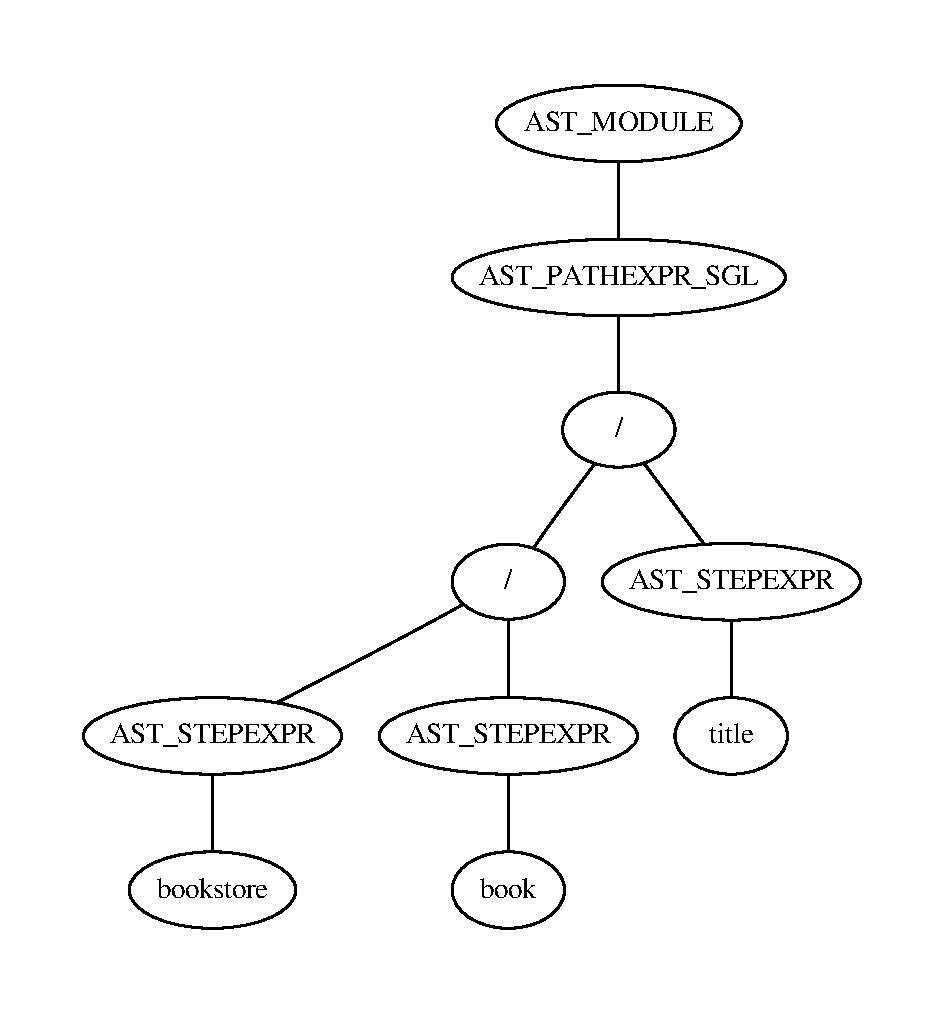
\includegraphics[width=0.4\textwidth]{img/graphs/path1}
\caption{Generated AST tree for a simple path expression}
\label{fig:discussion:ast:path1}
\end{figure}

This is one example of how to represent path expressions as tree structures.
With in-order tree traversal this tree should be fairly simple to reconstruct  
into the original path expression, as well as matching against a document object
model, or for performing staircase joins\cite{pathfinder_staircase}. Another  
proposed way to represent path expressions is the NoK (Next-of-Kin) tree
structure\cite{zhang_nok}, however NoK may be better suited for simple document
tree matching.

Further, the AST generated for a FLWOR query in figure \ref{tree:ast:flwor1}
(section \ref{sect:results:parser_output_ast}) can be represented in several
alternative ways that may be more suitable for loop-lifted staircase
joins\cite{pathfinder_staircase}. One such representation is
BlossomTree\cite{zhang_blossomtree}, which is tailored for representing
FLWOR-expressions which consists of multiple path expressions.

The representation of full-text queries is also a matter of interest. The
grammar is quite clear on operator and modifier precedence, however it may not
be obvious how to relate some modifiers (such as 
``\verb!with|without stemming!") to nodes. As seen in figure, we have simply
added this modifier as a child to the subject node. However, it could be
benefitial add this modifier as a sibling or parent node of the subject node
instead. This is a recurring design question with regards to several other
full-text modifiers, and will need further research for optimum AST
construction.

\subsection{Extendability and Data Flow Analysis}
\label{sect:discussion:ast:extend}
Currently the logic for scoping and symbol table lookups are embedded in the
grammar. It would be benefitial to have this logic removed and decoupled and
rather develop a data flow analysis framework with the necessary facilities for
performing scoping, symbol table lookup, as well as type inference and type
checking. The current implementation of scoping and symbol tables (described in
section \ref{sect:impl:scoping_and_symtab}) is adequate, however adding more
features could severly affect the readability and clarity of the grammar.


% ERROR HANDLING
\section{Error Handling}
\subsection{Syntax errors}
\label{sect:error_handling:syntax_errors}
As mentioned in section \ref{sec:impl:errorhandling}, error handling was added
by forcing ANTLR into throwing exceptions upwards to the calling program.

However, it quickly became appareant that some of the errors in the lexer were
not discovered by the parser, and no exceptions were thrown for these errors. The
lexer would simply print an error message to stderr, consume the offending
character, and attempt recovery. This led to complications when running the
XQuery Test Suite (see section \ref{sect:tests:manual}).



\section{Scoping and symbol tables}
Scoping was implemented using a simple tree structure consisting of parent- and
child scopes. XQuery only allows new scopes to be defined through the
enclosedExpr production rule. This makes it trivial to start a new scope at the
beginning of a enclosedExpr, and end the scope and the end of an enclosedExpr.
This has been implemented as follows:
\begin{figure}[!h]
\begin{verbatim}
enclosedExpr : 
    LBRACESi {
        Scope parent = this.currentScope; 
        this.currentScope = new Scope(); 
        this.currentScope.setParent(parent); 
    }
    expr 
    RBRACSi { 
        this.currentScope = this.currentScope.getParent(); 
    }
;
\end{verbatim}
\caption{Scoping logic embedded in grammar definition}
\end{figure}

Where this.currentScope is a reference to the ``current'' scope in this
context. This member variable is initiated with an empty scope when an object
of the parser class is instantiated.

The implementation above (which is formatted slightly for brevity) will
automatically build a scope tree as the input is parsed.

The currentScope object, which is an object of type Scope, holds one reference
to a symbol table. The symbol table, which is a simple subclass of
java.util.HashMap, is not capable of performing symbol lookups throughout the
scope tree. This functionality is rather provided by the Scope class. This UML diagram
illustrates the relationship between the Scope, SymTab, and Symbol classes:
\clearpage
\begin{figure}[!h]
  \centering
    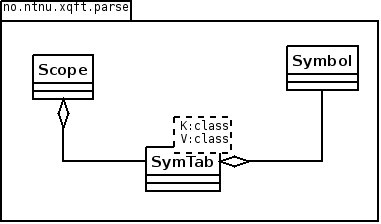
\includegraphics[scale=0.8]{img/uml1}
  \caption{Simplified UML overview of classes related to scope and symbol table}
\end{figure}

\section{Type checking}
XQuery/XPath has a well-defined type hierarchy.
\begin{figure}[h!]
  \centering
    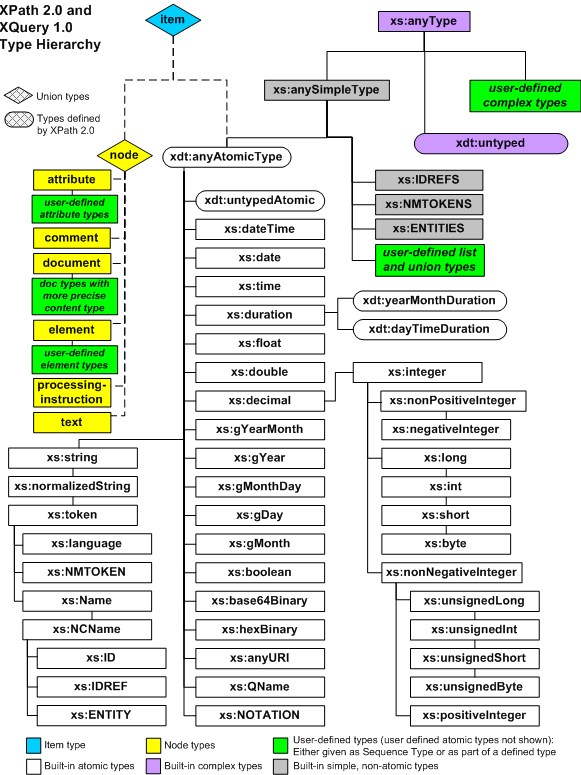
\includegraphics[scale=0.5]{img/xpathtypehierarchy}
  \caption{XQuery/XPath type hierarchy \cite{w3c04} (copyright
  \copyright W3C)}
\end{figure}
Here is a short overview of the basic type system:
\begin{itemize}
  \item Node types
    \begin{itemize}
      \item element()
      \item attribute()
      \item text()
      \item commment()
      \item document-node()
      \item processing-instruction()
    \end{itemize}
  \item Structure types
    \begin{itemize}
      \item Atomic types (xs:integer, xs:string, ..)
      \item Simple types (list, union)
      \item Complex types (user-defined types from an XML schema, except
      xs:anyType and xdt:untyped)
    \end{itemize}
\end{itemize}

Atomic types are strongly typed except xs:untypedAtomic, xs:anyURI, as well as
numerical types (xs:integer, xs:double, ..). Non-atomic simple types as well as
complex types are both strongly typed.

Proper type checking requires implementation of type inference and type
synthesis. This requires a stable abstract syntax tree and advanced data flow
analysis techniques to be feasible. Due to the inherent limitations in this
project, type checking has not been implemented - however the possibility of
this is discussed in section \ref{sect:summary:future_work}.

\underline{\textbf{\LARGE //TODO:}}
\begin{itemize}
  \item Dynamic vs. Static typing
  \item Strong vs. Weak (what and when)
  \item Type inference
  \item Michael Rys
\end{itemize}

\underline{\textbf{\LARGE //ODOT:}}

\section{Dead Ends}
\label{sect:discussion:deadEnds}
\underline{\textbf{\LARGE //TODO: Mads, om ikke du har noen p\aa~lager?}}



Hva har vi gjort som m\aa tte gj\o res om igjen?

\begin{itemize}
\item Skrive om dash: Validerende semantiske predikat, saa CharNotMinus etc
\item Feil splitting Lexer vs Parser, mye feilmeldingjakt
\item Keywords deklarert i @tokens -> vant alltid.
\item NCName med syntaktiske predikat
\end{itemize}

/* Hentet fra implementation: \\
In the grammar specified by the W3C, all the productions (terminals and
non-terminals) all start with uppercase letters. Initially this caused some
confusion, because this grammar naturally generated a very big lexer and a very
small and non-functional parser. \\
*/

\underline{\textbf{\LARGE //ODOT:}}

% Discussion / Coverage test results
\section{Coverage Test Results}
\label{sect:discussion:coverageResults}
As noted in section \ref{sect:results:tests}, our coverage testing ended at 
99.3\%. We can compare this result to official results published by W3C, with
some  important constraints: as described in section \ref{sect:method:testing},
the coverage tests is limited by the fact that we can only execute the set of
tests that are applicable in parse-time (and not run-time), since our parser
does not have a backend which produces output to be returned and compared to
expected output. Neither is our parser capable of detecting semantics such as
typing errors. This means that the official results from W3C include a number
of tests that have not been run on our parser.

Further, the XQuery test suite does not contain any full-text tests. So the
full-text extension capabilities of our parser are left untested, leaving only the XQuery features.

As such, it is crucial to keep in mind that \emph{our test results are not directly
comparable with official results}. However, they give a fair indication of the
parsers abilities, seen from a relative point of view.

On a side note, the results from the \emph{parse-error} scenario tests
(described in  section \ref{sect:method:testing}) would be directly comparable.
However, W3C does not annotate their result summaries with associated scenarios,
so this proved to be difficult to investigate within our given time frame.

\begin{figure}[h!]
  \begin{center}
    \begin{tabular}{ |c | c | c | c | c | c | c | c | c | c | c | c | c | c | c | }
      \hline
      Anglo-DT        & BaseX           & Berkeley DB XML   & DataDirect XQuery \\ \hline
      14630 / 100\%   & 14532 / 99.3\%  & 14566 / 99.5\%    & 14593 / 99.7\%  \\ \hline \hline
      eXist-db        & Galax           & Qexo              & Qizx \\ \hline            
      14544 / 99.4\%  & 14555 / 99.4\%  & 14535 / 99.3\%    & 14620 / 99.9\% \\ \hline \hline
      Saxon-SA        & Sedna XML       & Stylus Studio     & xbird/open \\ \hline
      14637 / 100\%   & 14459 / 98.8\%  & 14593 / 99.7\%    & 12041 / 82.3\% \\ \hline \hline
      X-Hive/DB       & xq2xsl          & XQuantum          & \\ \hline
      14589 / 99.7\%   & 14588 / 99.7\%  & 14378 / 98.2\%    & \\ 
    \hline
    \end{tabular}
  \end{center}
  \caption[Official XQuery test suite results]{Official XQuery test suite
  results compiled from the test suite web site\cite{w3ctestresults}} 
  \label{figure:table:w3c_test_results}
\end{figure}

Figure \ref{figure:table:w3c_test_results} gives a basic overview of the current
tests results published by the W3C at the current time of writing.

One interesting byproduct of the coverage tests were the utility of using it to
find and fix previously unknown bugs quickly. As such, this test suite also
works well as a regression test, since any improvement to the parser should
never degrade our coverage result -- however, it is hard to tell if tests that
previously failed would pass along with an identical amount of previously
passed tests that would fail, leaving the coverage percentage as before even
though the actual result was changed drastically. This kind of pitfall could be
avoided by keeping detailed track of which tests fail and pass, and compare new
results to old results and inspect the difference.

Of the 12478 test queries run 84 failed. These failed test cases can be broken down as follows:
\begin{itemize}
\item 46 erroneous queries caught by ANTLRs default lexer error handling.
\item 12 errors allowed by the parser
\item 9 type cast errors
\item 9 white space errors.
\item 5 XML specifiaction nonconformaties were allowed.
\item 2 untimely state transitions
\item 1 UTF-16 query
\end{itemize}

The majority of the failed test are because exceptions are caught by the lexer and not forwarded, leaving the parser unaware of the error (section \ref{sect:discussion:error_handling}). The 12 errors allowed by the parser and the 9 type cast errors are not syntactic errors, as such, as they are allowed by the W3C EBNF grammar. This test also shows that our lexer is to liberal with where white space can and cannot occur. The reason the tests which allowed illigal XML syntax and the untimely state transition failed are discussed in section \ref{sect:future:knownBugs}.


\section{Lookahead}
\label{sect:discussion:lookahead}
Originally we were under the impression, incited by the W3C source \cite{createTokenizer}, that the W3C XQuery specification, and consequently, the W3C XQuery full-text specification, were expressed as LL(1) grammars. We experienced that this could not be true, as did Kang et.al.\cite{kang_xquery_diglib}. It turns out that W3C once had argued that the grammar was LL(1), but not the corresponding full-text version \cite{grammarIsLL1}. In the newest version of the specification, LL(1), or even LL, is not mentioned at all. About the a former version of the specification claiming the XQuery grammar (not full text) to be LL(1), Michael Dyck, once a member of the W3C full-text task force \cite{dyckIsTaskForce}, expresses\cite{dyckOnList}:
\begin{quote}
For one thing, the grammar as defined by the EBNF is ambiguous, and no ambiguous grammar can be LL(1). [\ldots] the claim must be that the grammar as defined by the EBNF and the precedence chart is LL(1). The problem then is that LL(1)-ness isn't defined for such a grammar.
\end{quote}
The same must hold true for the full text version, as it is an extension of XQuery.

That XQFT is at least LL(2) can be demonstrated by the fact that a single function call is a valid query, a query may start with a namespace declaration, which is on the form \verb!declare namespace...! and that \verb!declare! is a permitted function name. There is no way to left factorize these productions, if not one rendering the grammar complex and possibly containing redundancies.

After left factoring all productions applicable the grammar still is a minimum of LL(3). This can be seen in figure \ref{fig:notLL2}, which shows a syntacticly valid typeswitch expression according to the W3C specification. The value after a \verb!case! keyword in a typeswitch can be a \verb!NCName!, which with no reserved keywords can be the character sequence "sensitive". In this example the parser at the end of line two would not know if the tokens \verb!case! and \verb!sensitive! are full-text match options or the start of a new case clause.

\begin{figure}[h!]
\begin{Verbatim}
typeswitch($c) 
   case $c as comment() return $c ftcontains "x"
   case sensitive return $p
   case surname return $p ftcontains "x" case sensitive
   default return ()
\end{Verbatim}
\label{fig:notLL2}
\caption[A typeswitch shows the need for LL(3)]{An example of a typeswitch demonstrating the need for LL(3).}
\end{figure}

As the W3C reference test parser \cite{parserTestPage}, our parser, when parsing the typeswitch example query, would prefer the match option alternative, meaning that the query would fail.

Because we chose the parser controlled strategy, our system's correctness depends on the parser utilizing as small a lookahead as possible. At its current state the maximum lookahead is $2$, with the exception of some syntactic predicates that make use of three tokens. Of the results in section \ref{sect:discussion:manualCoverage} it is apparent that most state transitions happen at the right time, except for some corner cases. But to reach 100\% test coverage the overall lookahead will have to be reduced to $1$. 




